\chapter{Real-Time Weather Radar with CHORDS}
\label{sec:realtime}
% This whole section is super weak on math, but maybe that is OK
% It just doesn't translate well to papers and dissertations, for one thing
% But also, shows how little support there is for weather radar data
% if our one programmer is unwilling to add it, we are up a creek
% Still, as a survey, perhaps this discussion is important
The issues and solutions presented in this dissertation thus far can be applied to enhance the process of data discovery even further when introduced to workflows involving recent developments in cyberinfrastructure for data. 
To this point, the focus has been on developing methods for identifying interesting and relevant features in historical datasets. 
It is also important, however, to consider real-time data, and the implications of incorporating the aforementioned methods in real-time.

Perhaps some of the most important applications of weather data is in discovering what is happening in the moment, and in predicting what will be happening in the near future. 
The stated goals of many radar networks, including the CASA network and the WSR-88D NEXRAD system, are to provide up-to-the-minute understanding of the ever evolving meteorological systems, to provide disaster warning, transportation planning, and logistical support for people operating within those network coverage regions. 
The data is used as inputs to models to attempt to discern the near-future effects that weather might have at many geographic scales. 
There is an industrial arms-race among start-up and large companies alike to provide hyper-local data of increasing fidelity to capitalize on the financial benefits of providing weather information with lower error rates than competitors, with the added benefit ofdeveloping solutions to augment safety for the populace. 
And there is growing momentum among science communities to develop modern infrastructure to facilitate these goals, within the broader scope of improving the open source, research state-of-the-art.

It is with this last goal in mind that the National Science Foundation (NSF) created EarthCube. 
The EarthCube program has focused on developing an ecosystem where researchers and engineers could focus on the technical and social aspects of modernizing cyberinfrastucture in the geosciences, in tandem with NSF.
The Cloud-HOsted Real-time Data Services for the geosciences (CHORDS) project is the funded project under the EarthCube umbrella that is focused on developing solutions for cost-effective cloud-stored real-time data streaming \cite{kerkez2016cloud}.

This chapter is designed to explain the operating characteristics and functions of CHORDS, as well as the survey of research in integrating weather radar data with CHORDS as informing development of the project.
While Chapter \ref{sec:classifying} illustrates the value designing and deploying models in historical Data Discovery applications, there is also potential for application to real-time streams to provide semantic insights regarding pressing weather concerns, along with populating label databases as data is produced.
It is with this in mind that we survey the current state of the CHORDS project, and discuss its applications to the problem of weather radar data storage, visualization, analysis, and classification, as a way to inform continued development in this active project.

\section{CHORDS}
\label{sec:realtime_chords}
CHORDS in its current format functions as a conduit for managing time series data streams.
The system has been described in \cite{kerkez2016cloud}, but some summary is presented here.
The project developed as the result of an EarthCube workshop, where a group of scientists representing multiple disciplines and multiple universities determined the need for a cross-discipline, remotely accessible platform for handling real-time data streams.
Over the past 6 years, the CHORDS project has evolved and managed a number of use cases, including seismological\cite{jones2017implementing}, hydrological\cite{wong2016real}, and meteorological.
It is this lattermost application that is the focus of this analysis.

A CHORDS Portal is a web application, managed via Docker\footnote{\url{https://www.docker.com/}} containers, and consists of several endpoints.
A researcher manages their real-time stream by first specifying a Site, which is the geospatial location where instruments are placed. 
The instruments themselves are managed on the Instruments page, where a user can specify the properties observed (Variables), and encode information about the observed properties from relevant standards, like SensorML \cite{van2009using}.
The observations themselves, the Measurements, can be visualized via a time series plot illustrating recent data, or can be downloaded via the Data downloads page.
There is also a programmatic API available for REST commands to add data or download, allowing connection to headless servers.
As such, it is straightforward to stream data to plug-ins like Grafana\footnote{\url{https://grafana.com/}} to perform more advanced thresholding and compute relevant real-time statistics.

\section{Specific Gates with Radar and Ground Sensors}
\label{sec:realtime_specificgates}

While the limitations of the CHORDS database with respect to access and number of writes is unable to handle the high bandwidth radar data in an exhaustive, one-pixel-per-Instrument manner, there remains interest in specifying certain radar gate values in this manner.

A weather scan can be thought of as an image, and indeed, this is an appropriate and extremely valuable paradigm. 
However, each radar range gate can also be interpreted as a time series, for each radar variable, and as such can be used as its own CHORDS Instrument.
In this paradigm, each radar variable at a point of interest maps to a CHORDS Variable, and the CHORDS Site can be located in the center of the geospatial area of interest.
In order to managed the fact that each Instrument is in different actual locations, we can pass the latitude and longitude of the radar range gates as Variables themselves, where each measurement is constant.
This is a powerful concept, and has been presented by the author in \cite{gooch2017integration}.
A graphical outline of the CHORDS portal in this setup can be seen in Figure \ref{fig:realtime_chordsportal_specificgates_concept}.

\begin{figure}[h]
	\centering
	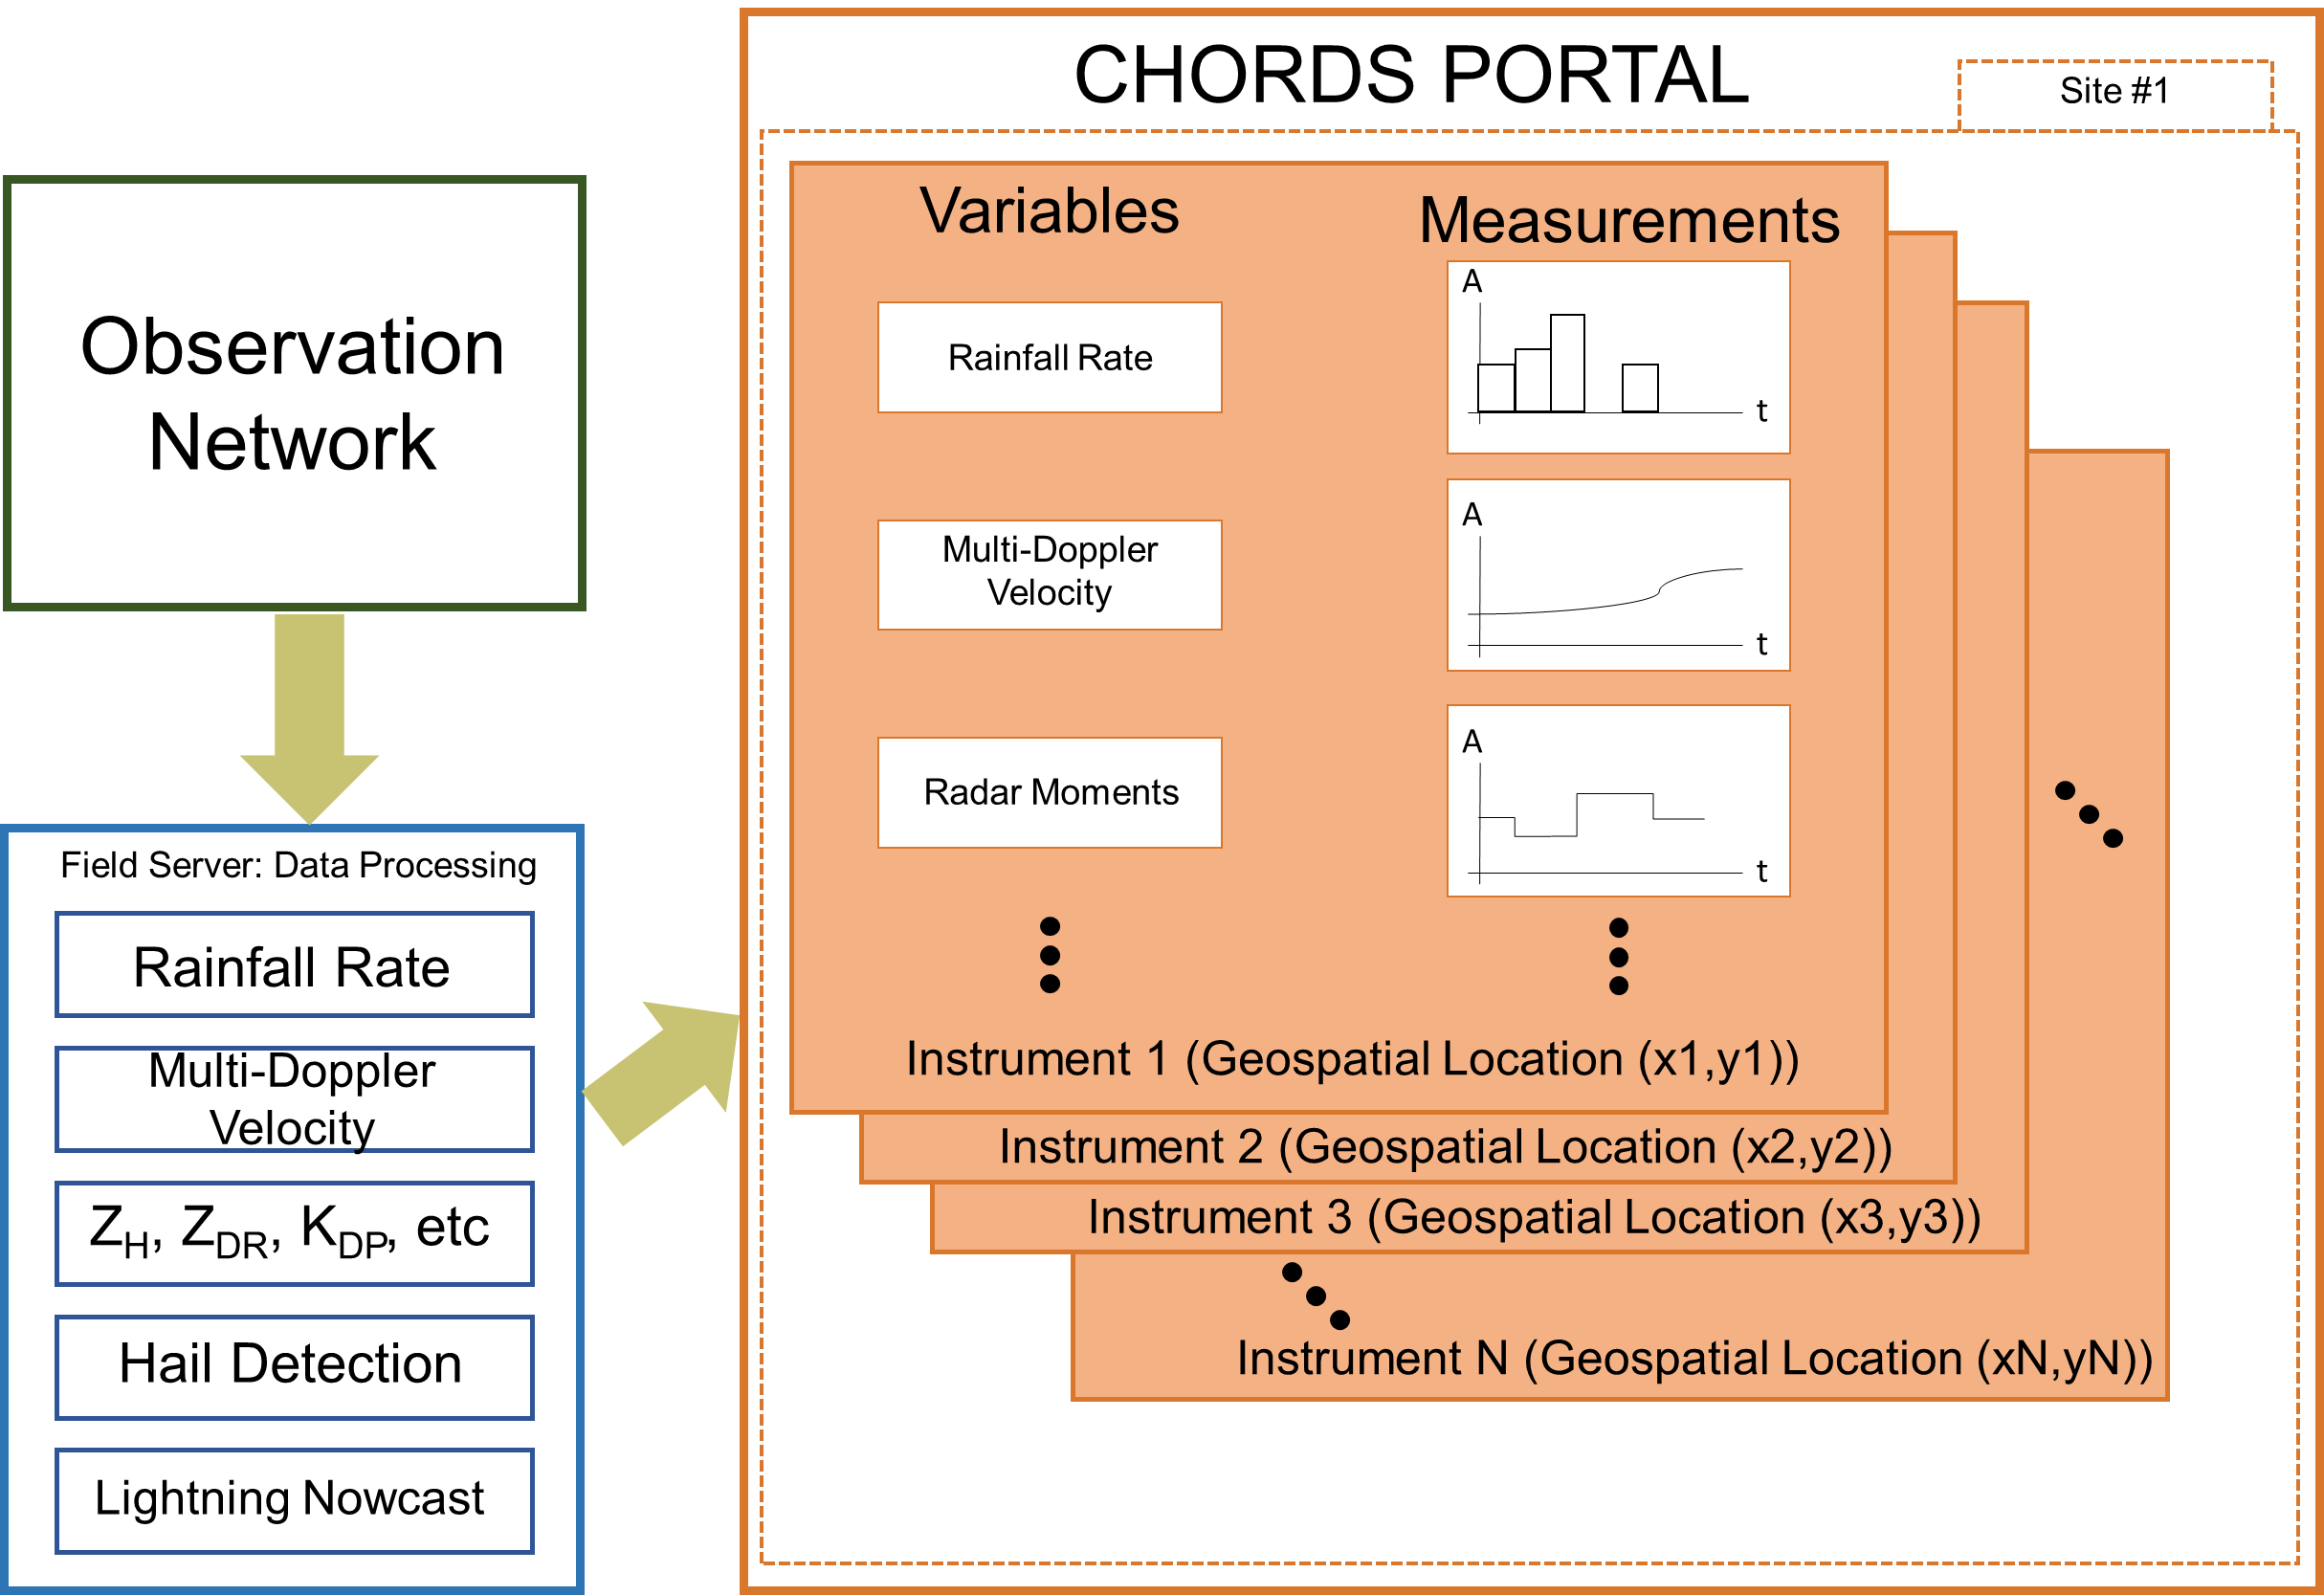
\includegraphics[width=\textwidth]{./thesis_code/plots/chords_portal_concept.png}
	\caption{CHORDS Portal, where selected radar range gates are used as Variables, allowing collocated ground sensors to stream data and provide direct ground-to-radar validation in real-time}
	\label{fig:realtime_chordsportal_specificgates_concept}
\end{figure}

The major gain here is that ground sensors collocated with these radar range gates can be streamed to the same Instrument, allowing real-time validation of either (or both) results.
This was tested using the hydrometeor classification product from the CASA DFW network and ground hail sensor data provided by Understory\footnote{\url{https://understoryweather.com/}}.
See Figure \ref{fig:realtime_chordsportal_hail} to see the benefit of such a setup.

\begin{figure}
	\centering
	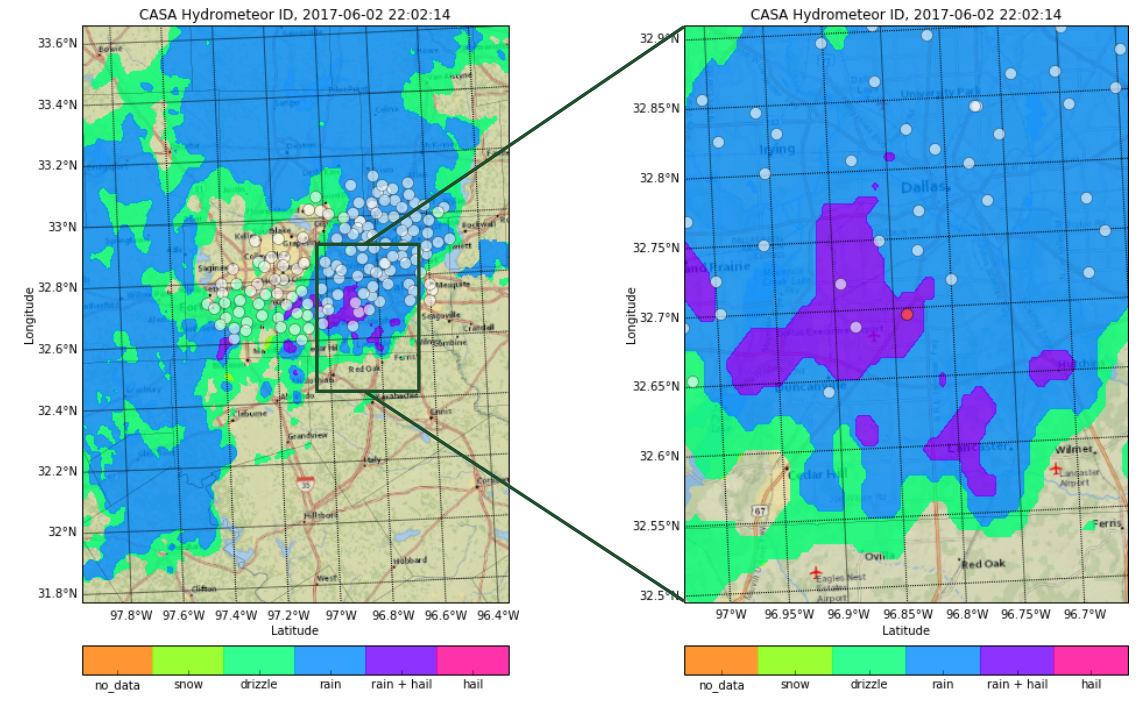
\includegraphics[width=\textwidth]{./thesis_code/plots/hail_radar_hid.png}
	\caption{Aligning hydrometeor identification product with hail sensor hits in the Dallas Fort Worth area, illustrating an example CHORDS use case}
	\label{fig:realtime_chordsportal_hail}
\end{figure}

\section{Full Image Support}
\label{sec:realtime_fullimage}

As of now, full image support has not been implemented, though this research has performed a substantive literature review and various experiments to inform the implementation of full radar image support.
Some of the key concepts and research are presented below.

\subsection{Data Storage}
\label{ssec:realtime_storage}

There are two reasonable methods for storing full radar data in a CHORDS portal.
The first is to simply post full NetCDF files containing completed volume scans.
One benefit to this method is that it opens up a host of potential plug-ins, and allows analysis and visualization of any radar variable.
However, the downside is that this represents an increase in storage footprint, and is a heavier load on server bandwidth.
The main alternative to this is simply passing pre-generated images, such as those presented above.
This is often done at radar operation centers in order to have a human-readable record of historical data, or as a method for generating reports.
As such, it represents lower overhead for the data generation and transmission.
Additionally, as has been shown in this work, there can be useful insight extracted from pre-generated data.
However, this does limit the kinds of analysis that can be performed as plug-ins to the CHORDS portal, and negates the possibility of cross-comparison to collocated instruments, one of the major gains in utilizing CHORDS portals in the preceding section.

\subsection{Data Analysis}
\label{ssec:realtime_analysis}
% Xarray + Dask, talk about how things like Spark and Pandas are great for structured data in tables, but as far as N-D radar data, few strong examples.
% Xarray is nice but unless you have access to tons of RAM, not faster than MATLAB for radar data processing like Zh vs Zdr plots, which would be nice to see in real time, or perhaps rain rate estimators, etc
% So many interesting avenues for real-time analysis, like twiddling sliders and buttons in a jupyter notebook, and populating statistics using most recent scans
% Perhaps too processing intense?

Increasingly, computing and data storage is managed in the cloud.
Various cloud storage and cloud compute platforms have arisen in recent years, leading to cyberinfrastructure developments in the way that data is analyzed.
Given the simplicity of storing data in the cloud, it is reasonable to extend CHORDS-managed data to plug-in to other cloud services.
For the N-dimensional datasets common in geosciences, including weather radar data, there are a few major toolkits worth mentioning:

\begin{itemize}
	\item Xarray\footnote{\url{http://xarray.pydata.org/en/stable/}}
	\begin{itemize}
		\item N-Dimensional array file I/O and analysis package in Python, designed as a NetCDF analysis toolkit. Allows labeled arrays, dataset management, and specification of dimensions, while providing tools for analyzing N-D data borrowed from popular tabular packages (such as pandas\footnote{\url{http://pandas.pydata.org/}})
	\end{itemize}
	\item Dask\footnote{\url{https://dask.org/}}
	\begin{itemize}
		\item Assists packages like Numpy and Xarray by providing straightforward parallelization of common numerical computing functions
	\end{itemize}
	\item Pangeo\footnote{\url{http://pangeo.io/}}
	\begin{itemize}
		\item Closely integrated with the two projects above, Pangeo is a project that seeks to reduce Time to Science for researchers needing to take advantage of cloud compute power, or supercomputers, for large scale analysis.
	\end{itemize}
	\item NetCDF-in-the-cloud
	\begin{itemize}
		\item Another EarthCube project, attempting to provide NetCDF storage to cloud-based data storage platforms
	\end{itemize}
\end{itemize}

\section{Deploying Image Classification in Real-Time}
\label{sec:realtime_classification}

To be added if CHORDS project supports full images in the near future.